%%%%%%%%%%%%%%%%%%%%%%%%%%%%%%%%%%%%%%%%%%%%%%%%%%%%%%%%%%%%%%%%%%%%%%%%%%%%%
%% MS LAYOUT - Pedro - 20 August 2005.
%% Revised version -   17 Dec    2006.
%% MS text moved to new file EcolLett. 22 May 2011.
%%%%%%%%%%%%%%%%%%%%%%%%%%%%%%%%%%%%%%%%%%%%%%%%%%%%%%%%%%%%%%%%%%%%%%%%%%%%%
\documentclass[a4paper,12pt]{article}
\usepackage{amsmath,amssymb}
%\usepackage[utf8]{inputenc}
%\usepackage[applemac]{inputenc}
\usepackage{geometry}
\usepackage{lscape}
\usepackage{setspace}
\usepackage{framed}
\usepackage{verbatim}
\usepackage{graphicx}                         
\usepackage{epstopdf}
\usepackage{booktabs}
\usepackage{natbib}
\usepackage{longtable}
\usepackage{rotating}                                                                                    
\newcommand{\tab}{\hspace{5mm}}
\usepackage{tabularx} 
\usepackage[margin=10pt,font=small,labelfont=bf]{caption}
\usepackage[left,pagewise]{lineno}
\usepackage{caption}
\usepackage{bibunits}
\DeclareGraphicsRule{.tif}{png}{.png}{`convert #1 `basename #1 .tif`.png}
\usepackage{fancyhdr} % This should be set AFTER setting up the page geometry
\pagestyle{fancy}     % options: empty , plain , fancy
\renewcommand{\headrulewidth}{0pt} % customise the layout...
\lhead{{\tiny Jordano \& Godoy - LDD events}}\chead{}\rhead{}
\lfoot{}\cfoot{\thepage}\rfoot{}
\setlength{\parskip}{\baselineskip} % increase paragraph separation
%%%%%%%%%%%%%%%%%%%%%%%%%%%%%%%%%%%%%%%%%%%%%%%%%%%%%%%%%%%%%%%%%% Title page
\begin{document}
\begin{bibunit}[science]
\title{Manuscript Draft\\
\vspace{2cm}
Extending the seed shadow: Long-distance dispersal of tree seeds by frugivorous animals}

\author{Pedro Jordano$^{\dag}$ and Jos\'e A. Godoy$^{\dag}$}

\date{Sevilla, \today}
\maketitle


\begin{spacing}{1.0}
$^{\dag}$ {\small Integrative Ecology Group, Estaci\'on Biol\'ogica de 
Do\~nana, CSIC, Pabell\'on del Per\'u, Avda. Mar\'ia Luisa, s/n, 
E-41013 Sevilla, Spain.}\\


{\small \textit{Corresponding author:} Pedro Jordano. Integrative Ecology Group, Estaci\'on Biol\'ogica de Do\~nana, CSIC, Pabell\'on del Per\'u, Avda. Mar\'ia Luisa, s/n, E-41013 Sevilla, Spain. Fax number: +34 95 4621125. Email address: jordano@ebd.csic.es}\\

\textbf{Key words}: dispersal kernel, fragmentation, frugivores, gene-flow, genetic neighborhood, long-distance dispersal, seed dispersal\\

{\small \textbf{Manuscript information: }** Words; ** Chars; ** Pages, * Figures; * Tables.}
\maketitle
\end{spacing}
\newpage
%%%%%%%%%%%%%%%%%%%%%%%%%%%%%%%%%%%%%%%%%%%%%%%%%%%%%%%%%%%%%%%%%%%% Abstract
\begin{linenumbers}
\begin{spacing}{1.5}
\begin{abstract}
Documenting long-distance dispersal events by frugivorous animals has been a challenge in seed dispersal studies \citep{Nathan:2003qe,Nathan:2006qy}. The difficulty to track movement patterns of animals and seed processing in the gut \citep{Mack:1995,Holbrook:2002fk,Holbrook:2006uq,Westcott:2005} has precluded attempts to directly estimate dispersal distances and made necessary resorting to estimates based on inverse modeling \citep{Clark:1999sv,Katul:2005yq,Nathan:2006}. Here we use multilocus microsatellite genotypes obtained from seed endocarps \citep{Godoy:2001} in combination with bayesian inference methods \citep{Wilson:2003gf} to assign the source population of dispersed seeds in a St Lucie's cherry population. We document long-distance dispersal by animals by showing that inter-population dispersal distances within a single reproductive episode can be as long as 17 km and represent up to 20 \% of the seeds. However, seed-mediated gene flow among these fragmented populations remains highly restricted, with most events of long-distance dispersal occurring among nearby populations. These are the first reliable long-distance estimates of seed dispersal among populations and are relevant to our understanding of connectedness among forest fragments and for predicting responses to habitat loss.
\end{abstract}
\end{spacing}
\end{linenumbers}
\newpage
%%%%%%%%%%%%%%%%%%%%%%%%%%%%%%%%%%%%%%%%%%%%%%%%%%%%%%%%%%%%%%%%%%% Main text
\begin{linenumbers}
\begin{spacing}{2}
\label{sect:intro}
Dispersal events of seeds and pollen assisted by animals are central ecological processes in many plant species, contributing to genetic structure, connectivity of metapopulations, and gene flow. While recent research on gene-flow patterns has emphasized pollen-mediated dispersal, especially for anemophilous species \citep{Ennos:2001ii,Sork:1999}, seed dispersal can be a major influence in plant population genetic structure because of its lasting effects on recruitment \citep{Ouborg:1999}. When frugivorous animals mediate in seed dispersal, unfrequent long-distance dispersal events (LDD) can occur consistently, i.e., repeatedly in successive reproductive episodes. Yet assessing the source and the dispersal vector for dispersed seeds sampled directly in the field is a lasting challenge in seed dispersal studies \citep{Nathan:2006qy} despite the fact that these are key parameters to understand animal-mediated dispersal. Both the results from inverse modeling \citep{Clark:1999sv} of the seed shadows (i.e., the spatial, landscape pattern of seed distribution following seed dispersal, \citep{Sork:1999}) and the scarce evidence from direct field observation of frugivore movements contributed to the widely admitted tenet of limited dispersal by frugivorous animals when compared to dispersal by wind \citep{Oddou-Muratorio:2001}. The results might appear contradictory with indirect inferences of long-distance seed dispersal events, generally mediated by  large frugivorous animals \citep{Fragoso:1997,Holbrook:2002fk,Holbrook:2006uq,Westcott:2000}, involving some times successful long-distance dispersal and dispersal to oceanic islands. The frequency distributions of animal-mediated seed dispersal distances are characterized by fat tails that render rigorous modeling deceptively limited \citep{Jordano:2007,Jordano:2007a,Nathan:2006qy}. Despite our ability and recent advances \citep{Godoy:2001,Garcia:2006,Jordano:2007,Hardesty:2006lr,Jones:2005fk_E31.7321} to document such sporadic events of successful long-distance dispersal, a serious limitation for further developments stems in our inability to estimate their frequency. Thus, predicting the frequency of dispersal \texttt{>}100 m, and specially the detection of among-population dispersal, is seriously  constrained by current methods. The inferences from seed trap  data alone \citep{Clark:1999sv} or seed marking studies \citep{Levey_etal_E31_7300}, rely on spatially limited sampling designs, and are limited by the difficulties in fitting the dipersal functions for the tail of the distribution \citep{Nathan:2003qe,Jordano:2007a}. Therefore, a serious methodological and conceptual challenge in seed dispersal studies has been the robust characterization of the frequency and extent of long-distance dispersal events.

Assessing who moves seeds where and which are the sources of these seeds (e.g., the population and maternal tree sources) is a key question in dispersal studies. When this information is available, reliable reconstructions of the seed dispersal kernels can be achieved (i.e., the total dispersal kernel) \citep{Nathan:2003qe,Jordano:2007a}. The connectedness among population fragments can be determined by combining these type of direct estimates of seed-mediated gene flow and spatially-explicit analysis of landscape connectivity \citep{Urban:2001}. 

By using hypervariable microsatellite markers with DNA amplified from the maternally-inherited endocarp seed tissue \citep{Godoy:2001} we have been able to ascribe the tree of origin for animal dispersed seeds within a population of \textit{Prunus mahaleb} (Rosaceae), an endangered species in SE Spanish mountains. Dispersal of this tree is mediated by a diverse coterie of frugivores, among which small-sized passerines (\textit{Sylvia} warblers, \textit{Turdus} thrush species, and redstarts \textit{Phoenicurus} spp.) predominate, together with carnivorous mammals \citep{Jordano:2000EcolMon}. Recently we showed that seed dispersal from other populations into a focal population can be substantial, and contributed differentially by a distinct subset of frugivore species, namely the largest sized ones \citep{Jordano:2007}.
% Need to re-write this par. with new updated data on samples...
We sampled seeds in seed traps laid out in a network of 20 sampling points including the major types of microhabitats in the forest (\textit{20}), throughout a ca. 21 ha plot including a large \textit{P. mahaleb} population (NCH, Fig. 1A) with 196 adult trees. Traps passively sampled seeds defecated or regurgitated by frugivores. All the adult trees in the population were genotyped for 11 microsatellite (simple sequence repeat, SSR) loci from leaf-extracted DNA. In addition, we sampled 192 trees from other 8 populations in the study area (Fig. 1A), totaling 388 trees genotyped. We assigned the maternal tree of origin for each of 95 seeds sampled in 1996 based on a direct comparison (identity check) of the multilocus genotype of each seed endocarp with the genotype of each of the adult trees, obtained from leaf tissue (\textit{10}). This method resulted in unambiguous direct estimates of the within-population seed dispersal distances for \textit{N}= 85 (89.47\%) of the seeds sampled in NCH that had the maternal source tree in this population. An ambiguous assignment of 2 seeds was due to failed amplification of 2 loci for these endocarps and was resolved by assigning the source to the nearest tree (see Suppl. Material).

Most of the dispersal events involving the within-population movement of seeds were within 25 m from the source maternal trees (Fig. 1B, \textit{10}). The remaining \textit{N}= 10 seeds (10.53 \%) are attributable to long-distance dispersal from other populations. We used assignment tests (\textit{21}) applied to the sample of 10 seeds unassigned to NCH trees to estimate the expected frequency of the seed endocarp multilocus genotype in each of 8 neighboring populations over an area of 30 x 25 km (Fig. 1A). We assigned each seed to the population with the highest log-likelihood of occurrence (Fig. 1A). Most seeds (6 out 10) came from populations CL and PCL, located at 3.2 and 1.2 km, respectively, from NCH (Fig. 1A). The remaining 4 seeds came from two relatively large populations (TC, with 100-150 trees, and NN having \texttt{} 1000 trees) located in a different watershed (Fig. 1B). Accounting for the area covered by \textit{P. mahaleb} trees in each population, we estimated the distances from the center of each population to be * km for TC and 6.4 km for NN. In contrast, we did not detect seed input from other nearby populations (e.g., CT, RH, Fig. 1B).

We are not aware of previous direct estimates of long-distance seed movement mediated by frugivorous animals and incorporating among-population dispersal. Our data extend the seed shadow of \textit{P. mahaleb} in a single reproductive episode up to a minimum of 6.4 km from the focal population and demonstrate that long-distance dispersal events are not infrequent yet very restricted to close populations. If frugivores track the temporal availability of fruits at different elevations (\textit{22, 23}), this might cause restricted possibilities for seed exchange among fragmented populations, even at close distance, that occupy different elevations (\textit{10}) and explains limited dispersal despite thorough removal of fruits by frugivores. Our data also suggest that the interchange of seeds is not symmetric among each pair of populations. The probability of NCH seeds being dispersed to CAL or PCAL should be much higher than the inverse, primarily because of the large difference in population size. Thus, we had evidence that seeds from the large NN and TC populations arrived in NCH in this particular reproductive event, despite being located at long distance and in a different watershed.

Animal frugivores are efficient in removing \textit{P. mahaleb} seeds and should contribute significantly to the connectedness of the fragmented populations via seed-mediated gene flow. The within- and among-population seed dispersal distances we document here are considerably larger than those reported previously for animal-dispersed species (\textit{5, 18, 24, 25}) and for breeding unit areas derived from pollen dispersal studies (\textit{14}). Previous analyses of the pollen and seed components of gene flow (\textit{12, 26-28}) have emphasized the former, probably due to the fact that most species examined had not endozoochorous dispersal and to the difficulty of reliably assessing seed dispersal events unambiguously, especially the long-distance ones. Using hypervariable molecular markers to jointly track seed dispersal patterns and to analyze open-pollinated progenies will help to clarify the relative contributions of seed and pollen movement to total gene flow. This will facilitate realistic modeling of dispersal functions incorporating the ubiquity and relative temporal frequency of long-distance dispersal events. In addition, our results emphasize the importance of considering the cascading, pervasive, effects of frugivore extirpartion from natural communities, where they play an important role in keeping the connectedness among population fragments and thus have a pivotal role for population recovery following perturbations.

\end{spacing}
\end{linenumbers}
%%%%%%%%%%%%%%%%%%%%%%%%%%%%%%%%%%%%%%%%%%%%%%%%%%%%%%%%%%%% Acknowledgments
\begin{linenumbers}
\begin{spacing}{1.5}
\section*{Acknowledgments}
\label{sect:ackn} We are indebted to Manolo Carri\'{o}n, Juan Luis Garc\'{\i}a-Casta\~{n}o, Jes\'{u}s Rodr\'{\i}guez, Cristina Garc\'{\i}a and, especially, Juan Miguel Arroyo for generous help with field and laboratory work and making possible this study. We appreciate the help and advice of Albert Abbott, Graham King and Amy Iezzoni, who generously provided \textit{Prunus} microsatellites before publication. Discussions with Cristina Garc\'{\i}a, Juan Miguel Arroyo, Eugene W. Schupp, Janis Boettinger, Jordi Bascompte, R\'{e}my Petit, Arndt Hampe, Alfredo Valido, and Carlos Meli\'{a}n were very helpful during the final stages of the manuscript. The study was supported by the Spanish Ministerio de Ciencia y Tecnolog\'{\i}a (BOS2000-1366-C02-01, REN2003-0273, and CGL2006-00373 to PJ). The Agencia de Medio Ambiente, Junta de Andaluc\'{\i}a, provided generous facilities that made possible this study in the Sierra de Cazorla and authorized our work there.
\end{spacing}
%\newpage
%%%%%%%%%%%%%%%%%%%%%%%%%%%%%%%%%%%%%%%%%%%%%%%%%%%%%%%%%%%%%%%%%% References
%\section{References}
%%% Literature Cited for main text
%\bibliographystyle{science} % Choose Science style for bibliography
%\bibliography{MS_Longdist}
\putbib[bu1]
\end{linenumbers}
\end{bibunit}
%%%%%%%%%%%%%%%%%%%%%%%%%%%%%%%%%%%%%%%%%%%%%%%%%%%%%%%%%%%%%%%%%%%%%%%%%%%%%

%%%%%%%%%%%%%%%%%%%%%%%%%%%%%%%%%%%%%%%%%%%%%%%%%%%%%%%%%%%%%%%%%%%%%% Tables
%\newpage
%section*{Tables}
\label{sect:tabl}
%%%%%%%%%%%%%%%%%%%%%%%%%%%%%%%%%%%%%%%%%%%%%%%%%%%%%%%%%%%%%%%%%%%%% Figures
\newpage
%%%% Figure LEGENDS

\textbf{Figure legends}\\

\textbf{Figure 1}. A. Map of the study area (located in the SE limit of Ja\'{e}n province, SE Spain- thick black line; thin lines, main streams and rivers) showing the 9 populations studied. Seeds sampled in the Nava de las Correhuelas focal population (NCH) and not assigned to the local trees growing there (N= 117 seeds, 1996 and 1997 seed crops) were tested for provenance from 8 populations in the region located within 1.5-20 km distance from the focal population. Numbers refer to the number of seeds assigned to each of the surrounding populations. B. The seed dispersal curve of \textit{Prunus mahaleb}, i.e., the frequency distribution of dispersal distances in a tree population (NCH, Nava de las Correhuelas) including the long-distance, among-population, dispersal estimates. The abcissa shows the actual distance values between the location of a dispersed seed (defecated or regurgitated by a frugivore) and its maternal tree (log-scale, actual distance + 1 m). At distance 0 m we represent seeds falling beneath the canopy of the mother tree. The inset shows the frequency distribution of dispersal distances within the population (i.e., not including seeds originating from other populations).\\ 

%%%%%%%%%%%%%%%%%%%%%%%%%%%%%%%%%%%%%%%%%%%%%%%%%%%%%%%%%%%%%%%%%%%%% FIGURES
%------------------------------------------------------------------- Figure 1
\begin{sidewaysfigure} 
\centering
%\centerline{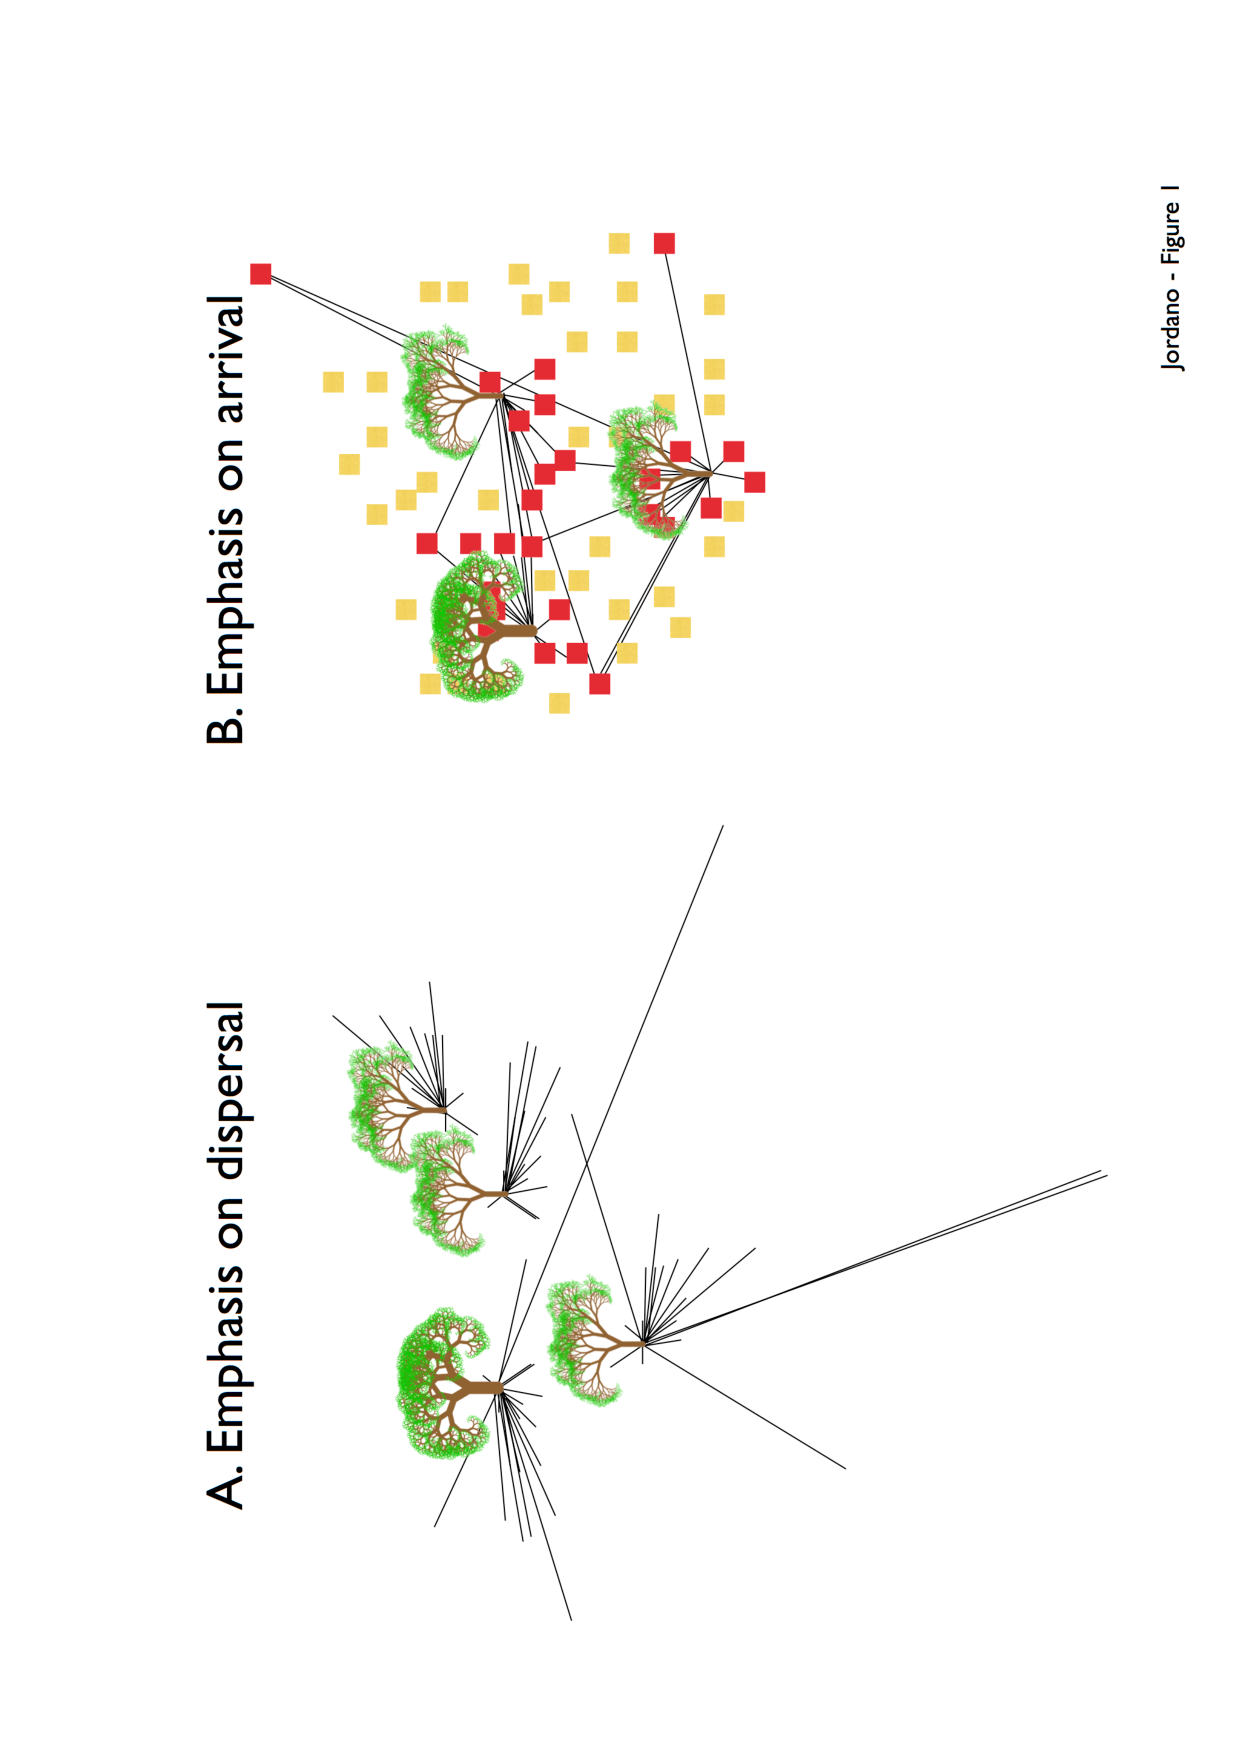
\includegraphics[height=11cm]{Fig1.pdf}} 
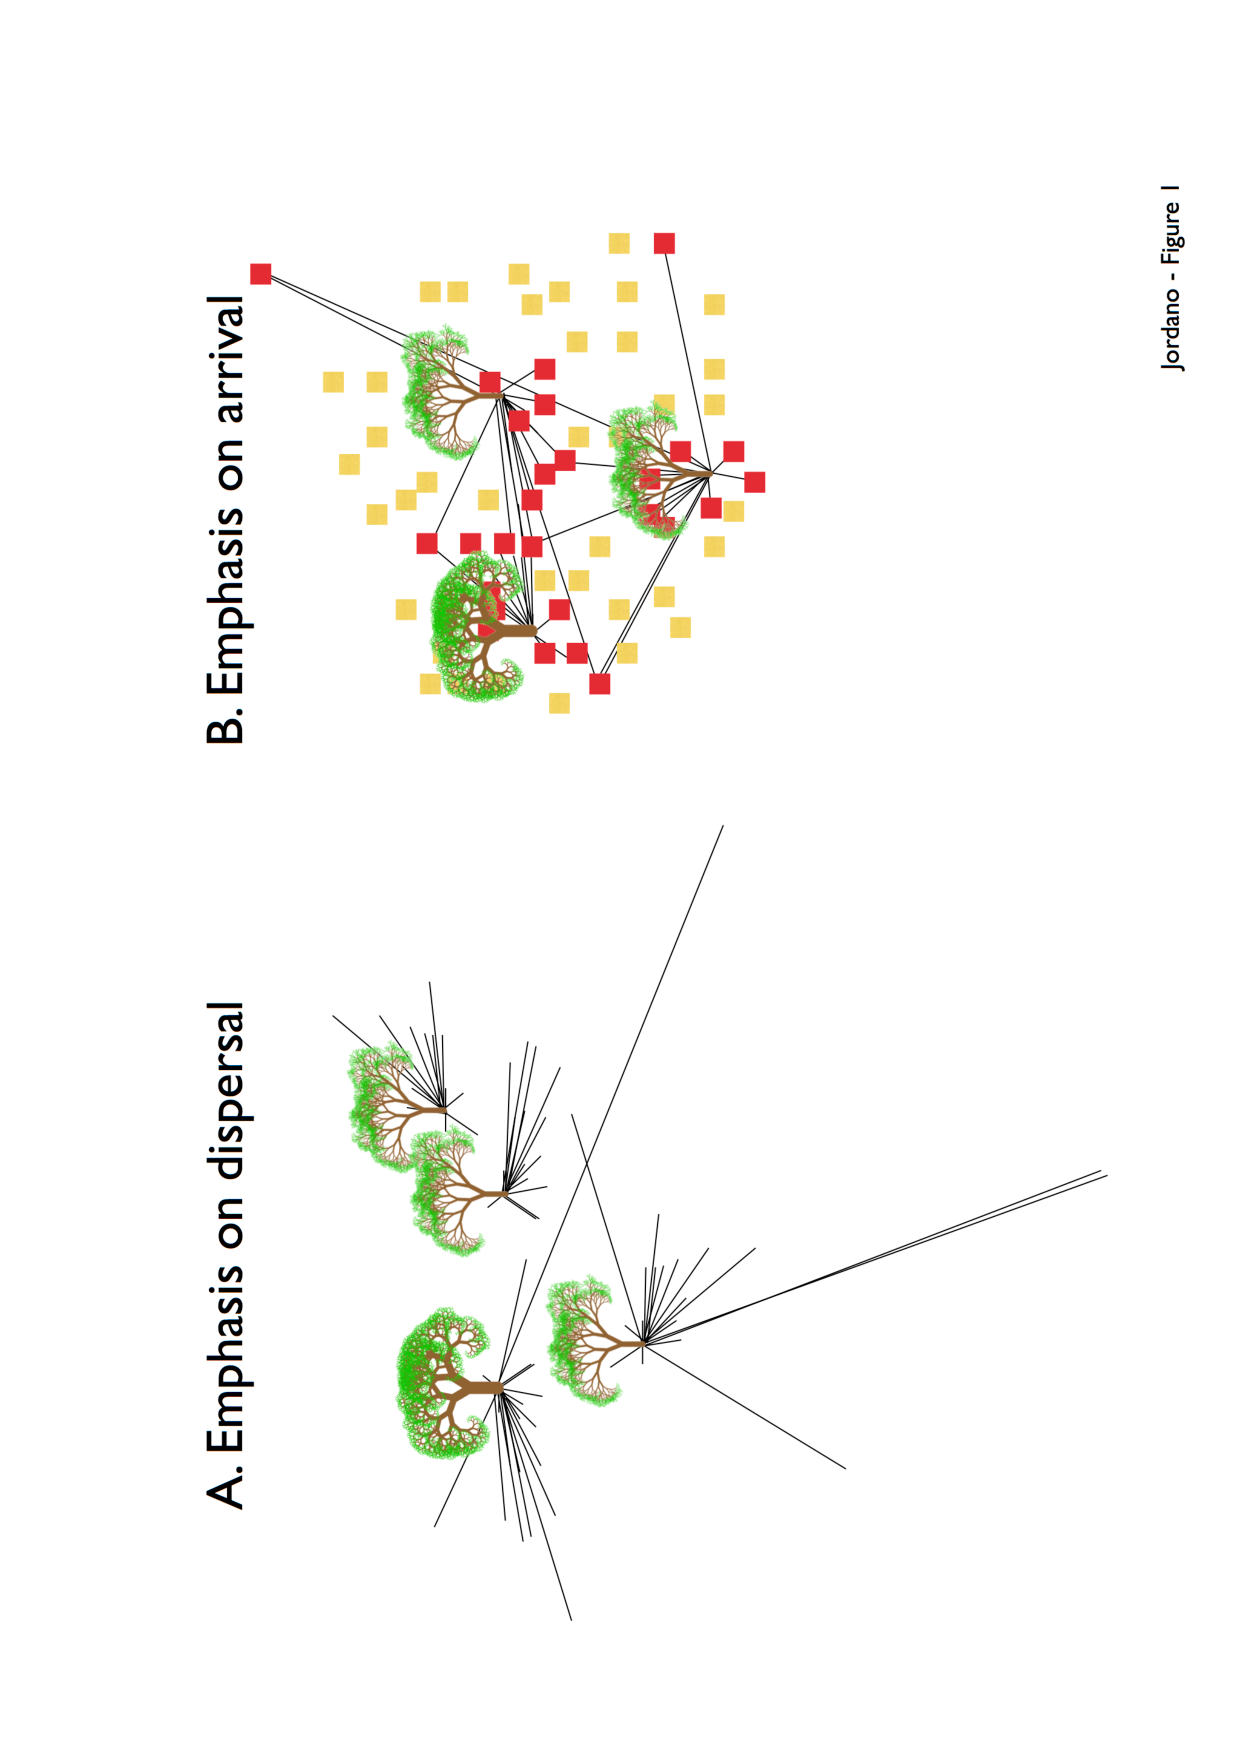
\includegraphics[height=15.5cm]{Fig1.pdf}
\end{sidewaysfigure}

%%%%%%%%%%%%%%%%%%%%%%%%%%%%%%%%%%%%%%%%%%%%%%%%%%%%% ONLINE SUPPORT MATERIAL
\newpage
\begin{bibunit}[science]
\section*{Online Support Material}
\begin{spacing}{2.0}
\textit{Methods}
A total of 9 local \textit{Prunus mahaleb} populations were selected  for analysis, all them in Parque Natural de las Sierras de Cazorla,  Segura y Las Villas (Ja\'{e}n province, SE Spain). In this area \textit{P.  mahaleb} naturally occurs as isolated small (10 trees) to medium-size  (150 trees) distinct populations. The main study population was  located in Nava de las Correhuelas (NCH), at 1615 m elevation. Detailed  descriptions of the area and general methods can be found in  \citep{Jordano:1994,Jordano:1995,Jordano:2000EcolMon,Jordano:2002}. We genotyped 388 trees, including all the 196 adult  trees from the main study site, NCH, increasing our previous  sample for this population (\citep{Godoy:2001}). Details of the extraction  and amplification protocols can be found in \citep{Godoy:2001,Jordano:2002}.

Seeds dispersed by animals were sampled by setting 20 replicates  of 2 seed traps each at different randomly-chosen locations in NCH population: beneath \textit{P.  mahaleb} trees (5 trees), beneath high shrubs (10 locations),  and benetah pine trees (5 locations) either with or without juniper  understory \citep{Godoy:2001,Jordano:2002}.

To assign the source tree for each dispersed seed we carried  out an identity check by matching the multilocus genotype of  the endocarp at 9 loci with those of the adult trees; for the  adult trees we assessed 11 SSR loci \citep{Cipriani:1999,Sosinski:2000}. We used CERVUS (\textit{9}) to identify the mismatches and multiple-matches among  endocarps and putative source trees. All the seed endocarps except  2 (among those matching NCH tree genotypes) were assigned to  a single tree in NCH; ten endocarps were not assignable to any  tree in NCH. The two seeds with double matching have failed amplifications  for two loci and resulted in ambiguous matchig with two putative  maternal trees. We assigned the seeds to the tree nearest to  the sampling location, due to the fact that this procedure would  minimize the estimation errors of dispersal distances when these  are distributed with high skew, i.e., a missasignment of a rare long-distance event would seriously bias the estimate of the dispersal function.

To assing the population of origin for the seeds not matched  by any tree in NCH we used a maximum-likelihood test based on  the probability that each particular endocarp multilocus genotype  would be obtained in each of the 9 populations (excluding NCH).  The assignement proceeds as follows \citep{Wilson:2003gf,Beaumont:2004lr}: for each population  and locus, the relative frequencies of alleles are estimated  (\textit{p}$_{\mathit{il}}$\textit{, p}$_{\mathit{jl}}$\dots ); the expected probability of  a seed endocarp genotype is determined for each locus in that  population and these expected frequencies are muliplied across  loci. The endocarp genotype is assigned to the population with  highest log-likelihood of occurrence.\\

\end{spacing}
%%%%%%%%%%%%%%%%%%%%%%%%%%%%%%%%%%%%%%%%%%%%%% References for Online Material
\putbib[bu2]
\end{bibunit}
%%%%%%%%%%%%%%%%%%%%%%%%%%%%%%%%%%%%%%%%%%%%%%%%%%%%%%%%%%%%%%%%%%%%%%%%%%%%%
\end{document}

